
\documentclass[]{book}\usepackage[]{graphicx}\usepackage[]{color}
%% maxwidth is the original width if it is less than linewidth
%% otherwise use linewidth (to make sure the graphics do not exceed the margin)
\makeatletter
\def\maxwidth{ %
  \ifdim\Gin@nat@width>\linewidth
    \linewidth
  \else
    \Gin@nat@width
  \fi
}
\makeatother

\definecolor{fgcolor}{rgb}{0.345, 0.345, 0.345}
\newcommand{\hlnum}[1]{\textcolor[rgb]{0.686,0.059,0.569}{#1}}%
\newcommand{\hlstr}[1]{\textcolor[rgb]{0.192,0.494,0.8}{#1}}%
\newcommand{\hlcom}[1]{\textcolor[rgb]{0.678,0.584,0.686}{\textit{#1}}}%
\newcommand{\hlopt}[1]{\textcolor[rgb]{0,0,0}{#1}}%
\newcommand{\hlstd}[1]{\textcolor[rgb]{0.345,0.345,0.345}{#1}}%
\newcommand{\hlkwa}[1]{\textcolor[rgb]{0.161,0.373,0.58}{\textbf{#1}}}%
\newcommand{\hlkwb}[1]{\textcolor[rgb]{0.69,0.353,0.396}{#1}}%
\newcommand{\hlkwc}[1]{\textcolor[rgb]{0.333,0.667,0.333}{#1}}%
\newcommand{\hlkwd}[1]{\textcolor[rgb]{0.737,0.353,0.396}{\textbf{#1}}}%
\let\hlipl\hlkwb

\usepackage{framed}
\makeatletter
\newenvironment{kframe}{%
 \def\at@end@of@kframe{}%
 \ifinner\ifhmode%
  \def\at@end@of@kframe{\end{minipage}}%
  \begin{minipage}{\columnwidth}%
 \fi\fi%
 \def\FrameCommand##1{\hskip\@totalleftmargin \hskip-\fboxsep
 \colorbox{shadecolor}{##1}\hskip-\fboxsep
     % There is no \\@totalrightmargin, so:
     \hskip-\linewidth \hskip-\@totalleftmargin \hskip\columnwidth}%
 \MakeFramed {\advance\hsize-\width
   \@totalleftmargin\z@ \linewidth\hsize
   \@setminipage}}%
 {\par\unskip\endMakeFramed%
 \at@end@of@kframe}
\makeatother

\definecolor{shadecolor}{rgb}{.97, .97, .97}
\definecolor{messagecolor}{rgb}{0, 0, 0}
\definecolor{warningcolor}{rgb}{1, 0, 1}
\definecolor{errorcolor}{rgb}{1, 0, 0}
\newenvironment{knitrout}{}{} % an empty environment to be redefined in TeX

\usepackage{alltt}
\usepackage[english]{babel}
\usepackage{graphicx}
\usepackage{fancyref}
\usepackage{hyperref}
\usepackage[scale=2]{ccicons}
\usepackage{url}
% \usepackage{xmpincl}
% \usepackage[
%     type={CC},
%     modifier={by-nc-sa},
%     version={3.0},
% ]{doclicense}


% Title Page
\title{Analyzing data using linear models}


\author{St\'ephanie M. van den Berg}
\date{Version SPSS 1.0.0 \\ (\today)}
\IfFileExists{upquote.sty}{\usepackage{upquote}}{}
\begin{document}
\maketitle

\pagestyle{empty}
%% copyrightpage
\begingroup
\footnotesize
\parindent 0pt
\parskip \baselineskip


Copyright \copyright \space 2018 by St\'ephanie M. van den Berg \\
University of Twente\\
Department of Research Methodology, Measurement and Data Analysis\\
Licensed under Creative Commons, see https://creativecommons.org/licenses/\\
For source code and updates: github.com/pingapang/book\\
E-mail: stephanie.vandenberg@utwente.nl\\
\ccbyncsa

   

 

\begin{center}
\begin{tabular}{ll}
First edition:  & October 2018 \\
\end{tabular}
\end{center}




\endgroup
\clearpage












\chapter*{Preface}
This book is intended to be of use to bachelor students in social, behavioural and management sciences that want to learn how to analyze their data, with the specific aim to answer research questions. The book has a practical take on data analysis: how to do it, how to interpret the results, and how to report the results. All techniques are presented within the framework of linear models: this includes simple and multiple regression models, to linear mixed models and generalized linear models. All methods can be carried out within one supermodel: the generalized linear mixed model. This approach is illustrated using SPSS.



\tableofcontents





% knit_child('chapter_1.Rnw') % exploring your data, descriptive statistics
% 
% knit_child('linear modelling introduction.Rnw') % simple regression
% 
% 
% 
% 
% knit_child('chapter_inference_I.Rnw')
% 
% knit_child('chapter_inference_II.Rnw')
% 
% knit_child('chapter_multiple regression.Rnw') % multiple regression
% 
% knit_child('chapter_categorical.Rnw')
% 
% knit_child('chapter_6.Rnw') % moderation
% 


\chapter{Linear modelling: more advanced topics}\label{chap:advanced}


\subsection{Planned comparisons}

Suppose you have height data from three countries: Greece, Italy, and Norway. You might wish to know whether in these populations there is a difference in average height. If that is all you want to know, you can perform the SPSS UNIANOVA analysis described above. In that case, the null-hypothesis is
\\
\\
$H_0: \mu_{Greece}=\mu_{Italy}=\mu_{Norway}$
\\
\\
However, suppose your most important hypothesis is really much more specific: you only want to know whether the average height in Italy is different from the average height in Greece. The corresponding hypothesis would then be: 
\\
\\
$H_0: \mu_{Greece}=\mu_{Italy}$
\\
\\
In such cases, where the null-hypothesis is more specific than simply stating "there are differences among the groups", then you should perform \textit{planned comparisons}. Here you would like to make a comparison between the average heights of Greece and Italy You could also say you'd like to \textit{contrast} the average height of Greece with that of Italy. 

We then have to define this contrast in such a way that SPSS knows what we want. So we could define our contrast in a similar vein as the null-hypothesis. Let's call the contrast $\gamma_1$.
\\
\\
$\gamma_1: \mu_{Greece}=\mu_{Italy}$
\\
\\

This contrast could also be written such that there is zero on the right-hand side of the equation, like this:
\\
\\
$\gamma_1: \mu_{Greece}-\mu_{Italy}=0$
\\
\\
This is the preferred way of specifying contrasts: having a zero on the right-hand side. And how about Norway? How do we add Norway into this contrast? Well, notice that you could also write the contrast like this:
\\
\\
$\gamma_1: (1)\times \mu_{Greece} + (-1) \times \mu_{Italy} + (0) \times \mu_{Norway} =0$
\\
\\
So we could code this specific contrast with the numbers preceding the group means: A 1 for Italy, a -1 for Greece and a 0 for Norway. For SPSS therefore, to specify a contrast, we only need this coding. This can be done in the following way. Suppose you have data on height, summarized in the boxplot in Figure \ref{fig:fig1416}. Note that in this SPSS data set, the country variable is coded 1 for Greece, 2 for Italy and 3 for Norway. Then we could use the following syntax to ask for the specific comparison (or contrast) of the first and the second group, that is, Greece and Italy, respectively. So group 1 (=Greece) gets a 1, group 2 (=Italy) gets a -1, and group 3 (=Norway) gets a 0, so our coded contrast looks like $(1, -1, 0)$.



\begin{knitrout}
\definecolor{shadecolor}{rgb}{0.969, 0.969, 0.969}\color{fgcolor}\begin{figure}

{\centering 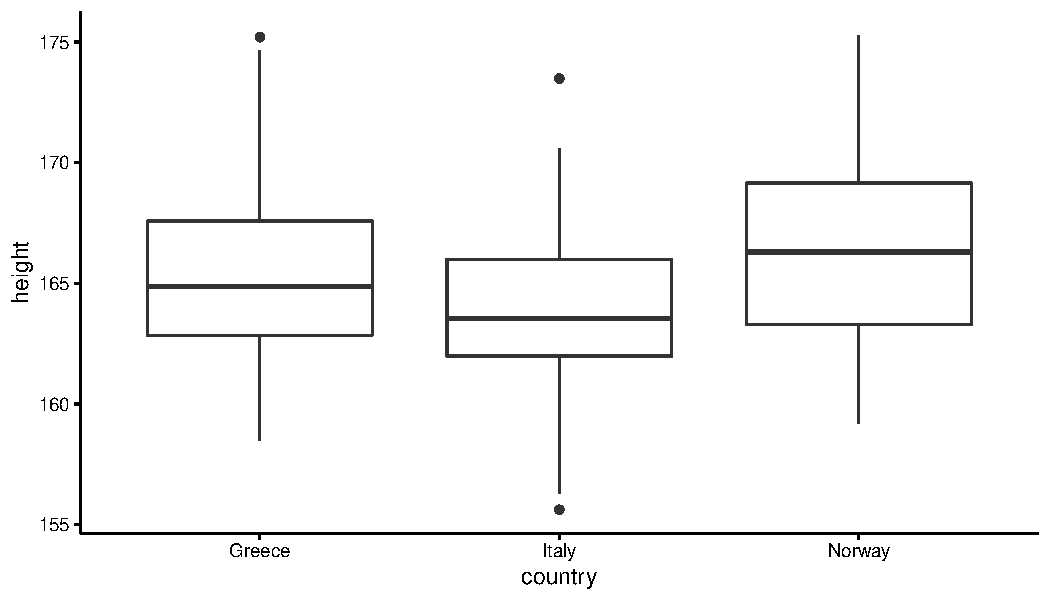
\includegraphics[width=\maxwidth]{figure/fig1416-1} 

}

\caption[Data on height in three countries]{Data on height in three countries.}\label{fig:fig1416}
\end{figure}


\end{knitrout}


\begin{verbatim}
UNIANOVA height BY country
/DESIGN=country
/CONTRAST(country)=SPECIAL(1  -1  0).
\end{verbatim}

In Figure \ref{fig:contrast1} we see the output. We see first that the general null-hypothesis that all three countries have the same average height is rejected, $F(2, 147)= 6.14, MSE=14.77, p = 0.003$. This test has 2 degrees of freedom, one for each of the two dummy variables that are needed to test this model. The error degrees of freedom equals 147: that is the number of data points (150) minus the number of parameters in the model: one for the intercept and two for the dummy variables, so $150-3=147$.


\begin{figure}[h]
    \begin{center}
       \includegraphics[scale=0.9,trim={0cm 11cm 0cm 0cm}, clip,width=0.7\linewidth]{/Users/stephanievandenberg/Dropbox/Statistiek_Onderwijs/Data" "Analysis/spss" "examples" "linear" "model/planned" "comparisons/contrast1.pdf}
    \end{center}
    \label{fig:contrast1}
    \caption{Output of the contrast analysis on height data from three countries.}
\end{figure}


Next, we see the results for our \textit{specific} null-hypothesis (the contrast): that the means for Greece and Italy are equal, irrespective of Norway. We see a Contrast Estimate of 1.008 and a significance level of $p=0.19$. So the contrast is positive: what does this mean? Well, let's put the 1.008 into our contrast above:
\\
\\
$\gamma_1: (1)\times \mu_{Greece} + (-1) \times \mu_{Italy} + (0) \times \mu_{Norway} = 1.008$
\\
\\
which can be simplified to
\\
\\
$\gamma_1:  \mu_{Greece} - \mu_{Italy}  =  1.008$
\\
\\
So the 1.008 indicates that the average height in Italy is 1.008 cm shorter than in Greece, at least in our sample. The relatively high $p$-value indicates that the population means are however not different: we do not reject the null-hypothesis that the average heights are the same.

We also see an $F$-test for this contrast, $F(1, 147)=1.721, MSE= 14.76, p=0.19$.
Since the first degrees of freedom number is a 1, we know that $F$ is the same as a squared $t$, $t^2$, So, an equivalent presentation of the contrast effect would be $t(147)=2.96, p=0.19$

Now perhaps you realize, why didn't we do a $t$-test in the first place? We might have taken the Greece and Italy data separately, used a dummy variable and then run an ordinary linear model. Well, let's see what would happen then.

First we let SPSS select only the Greece and Italy data with the SELECT IF syntax, and next run an UNIANOVA, using the BY keyword for country to indicate that we treat it as a categorical variable. We also let the selection be preceded by a TEMPORARY commmand, to indicate that the selection only applies to the analysis that follows.

\begin{verbatim}
TEMPORARY.
SELECT IF (country<3).
UNIANOVA height BY country
/DESIGN=country
/PRINT = PARAMETER.  
\end{verbatim}


In the output in Figure \ref{fig:simplettest} we see that now only the data from Greece and Italy are compared. From the Parameter Estimates table, we see that country 2 is the reference category, which is Italy. We also see that the average height in Greece is 1.008 cm taller than Italy. This effect is not significant, $t(98)=1.371,p=0.17$. We use 98 degrees of freedom because we have 100 people and loose 2 degrees of freedom, one for the intercept and once for the regression coefficient for country=1. Note that this number is also indicated in the Tests of Between-Subjects Effects table, as the df of the Error.

\begin{figure}[h]
    \begin{center}
       \includegraphics[scale=0.4]{/Users/stephanievandenberg/Dropbox/Statistiek_Onderwijs/Data" "Analysis/spss" "examples" "linear" "model/planned" "comparisons/simplettest.png}
    \end{center}
    \label{fig:simplettest}
    \caption{Output of an analysis after selecting only the data from Greece and Italy.}
\end{figure}

 

So what is different from the contrast effect? First of all, we see that the $p$-value is different: the $p$-value for the contrast effect analysis is somewhat larger than the one for the 'ordinary' $t$-test. Second, we see that the $t$-statistic is different: In the contrast analysis the $t$-value was 2.96 and in the ordinary analysis it was 1.371. So part of the reason that the $p$-value is different for the contrast is that the $t$-value is higher. Third, we see that the degrees of freedom has changed from 147 to 98. Well, we know that the significance level of a $t$-value depends on its size, the higher the $t$-value the lower the $p$-value, and we know that significance also depends on the degrees of freedom: the more degrees of freedom, the lower the $p$-value. 

So why has the $t$-value changed? Well, we know that the $t$-value is nothing but the regression coefficient divided by its standard error, $t=B/{SE}$. If we compare the two outputs, we see that the effect of $B$ is the same, the regression coefficient is equal to 1.008, and the contrast estimate in the Contrast Results (K-Matrix) is 1.008. So the sizes are the same. 

So the only difference between the two analyses can be the standard error. It turns out the standard error is computed in different ways: in the first contrast analysis, this SE is computed on the basis of \textit{all} the data, including the Norway data (150 people). We can see that from the degrees of freedom, the number of people minus 3. Why three? Because we also compute the variance of the Norway data, for which we have to estimate the mean (variance is the average squared difference from the mean). In the second analysis, we only used the data from 100 Greeks and Italians. The Norway data was not used at all, that's why the degrees of freedom is different and also the standard error for our $t$-statistic. 
\\
\\
Thus in summary: if we have a very specific hypothesis about the difference in means among two groups, it's better to use a contrast analysis, rather than a simple analysis regarding only those two groups. The reason for this is that \textit{more information is used}, even from groups for which we have no specific hypothesis. 
\\
Note that here we saw a higher $p$-value for the contrast analysis, but still, in general it is wiser to use as much data as possible, so we prefer a contrast analysis over a simple analysis excluding other groups.
\\
\\
The above example of comparing only the means of two groups, at the same time making use of the data in other groups, is called a \textit{simple contrast}. Now let's look at a \textit{complex contrast}. Suppose your hypothesis is that average height is different in Northern-European countries than in Southern-European countries, then you would like to know whether Italy AND Greece taken together differ regarding the average height from Norway. So we'd like to compare the average height in Norway to the average height in Greece and Italy together. We could write that null-hypothesis as follows:

\begin{eqnarray}
H_0 : \frac{\mu_{Greece}+ \mu_{Italy}}{2} = \mu_{Norway}
\end{eqnarray}


In other words, the mean height in Norway is equal to the \textit{average} mean height in the two other countries. If we want to test this hypothesis, we have to define a contrast. So we get the zero on the right-hand side in the following way:

\begin{eqnarray}
\gamma_2 : \frac{\mu_{Greece} + \mu_{Italy}} {2} - \mu_{Norway}  = 0 
\end{eqnarray}


This in turn we can write as 

\begin{eqnarray}
\gamma_2 : 0.5 \mu_{Greece} + 0.5 \mu_{Italy} - 1 \mu_{Norway}  = 0 
\end{eqnarray}


In SPSS, we can code this in the following way $(\frac{1}{2} \frac{1}{2} -1)$\footnote{Note that for the SPSS variable country variable, the first group is Greece, the second is Italy and the third is Norway. The contrast code should reflect the same order.}. We use the following syntax:

\begin{verbatim}
UNIANOVA height BY country
/DESIGN=country
/CONTRAST(country)=SPECIAL(0.5  0.5  -1).
\end{verbatim}


Now let's compare this analysis where we use a dummy variable NrthrnEr, where we code 1s for Norwegians and 0s for Greeks and Italians. We then run an ordinary linear model on the data using this dummy that is a quantitative predictor of height:


\begin{verbatim}
UNIANOVA height WITH NrthrnEr
/PRINT=PARAMETER
/DESIGN=NrthrnEr.
\end{verbatim}

From the contrast analysis we obtain $F(1,147)=10.56, MSE=14.77, p=0.001$, which is equivalent to $t(147)=3.25, p=0.001$. From the dummy variable analysis, we obtain $t(148)= 3.24, p=0.001$. So in this case, the results are very close: the degrees of freedom is larger for the dummy variable analysis, but the $t$-value is lower. All in all, we gain nothing much, and that is because in the dummy analysis we also use all of the data: we put the Greeks and Italians in one group (N=100), and the Norwegians in another group (N=50). The degrees of freedom therefore differs cause we only need to estimate 2 means in the dummy analysis, instead of 3 in the contrast analysis.

In general: if you run a model where you compare various groups, AND you have very specific hypotheses that you'd like to test, it is generally advised to run a contrast analysis, including a small number of them, and then report only the tests and $p$-values of those contrast. Do not then also report the $p$-values of the parameters of your model. Actually, your contrasts are a respecification of your model: either report the contrasts or the parameters, but not both, since they contain the same information. If you report too many $p$-values, the probability that you make a Type I error (concluding that you have a significant difference while there is really no difference) becomes too large. That is also the reason why you should report not more contrasts than the number of your parameters for your variable. For example, if you compare 5 groups, you will have 4 parameters for these groups. In that case specify no more than 4 contrasts. SPSS has a number of prespecified sets of contrasts, like Helmert, Deviation, Difference, etcetera. Check out the SPSS manual for more details. If you want something more specific, use the SPECIAL option as indicated above. 

Also very important: only go for contrasts when the overall ANOVA is significant. If the group means are not significantly different from eachother in a general sense, it is generally not advised to test specific contrasts.

\subsection{Testing more than one contrast}

In some cases you have a number of research hypotheses about group differences. For instance, you might have the a priori hypothesis that people in Northern countries are taller than in Southern countries, and another a priori hypothesis that people in Western countries are taller than in Eastern countries. So, a priori you have the hypothesis that the mean height in Norway is different from the mean heights in Greece and Italy combined. Second, you expect that the mean height in Italy is higher than in Greece.

You could test these two hypotheses at once in SPSS by specifying a $K$ matrix, like so:

\begin{verbatim}
UNIANOVA height BY country
/DESIGN=country
/CONTRAST(country)=SPECIAL(-0.5  -0.5  1
                            1    -1   0).
\end{verbatim}

Remember that the countries were coded like 1=Greece, 2=Italy, and 3= Norway. So the first null-hypothesis that is tested is that Norway has the same mean as the average of Greece and Italy. The second null-hypothesis is that Greece and Italy have the same mean.

This set of contrasts is said to be \textit{orthogonal}: whether or not we find a significant result for the first contrast has nothing to do with whether we find a significant result for the second contrast. Why this is the case can be seen from the $K$ matrix: if we take the first elements of the first and second row and multiply them we get $-0.5 \times 1 = -0.5$. If we take the second elements of the first and second row and multiply them we get $-0.5 \times -1 = 0.5$. If we take the third elements of the first and second row and multiply them we get $1 \times 0 = 0$. If we add these numbers we get $-0.5 + 0.5 +0= 0 $. Here we get a total of 0, which indicates that the contrasts are orthogonal, implying that the statistical results for contrast 1 and 2 are independent of eachother. If the sum is unequal to 0, the contrasts are said to be \textit{dependent}. 
Here's an example of a non-orthogonal set of contrasts:

\begin{verbatim}
UNIANOVA height BY country
/DESIGN=country
/CONTRAST(country)=SPECIAL( 1    0   -1
                            1   -1   0).
\end{verbatim}

Here the sum of the products equals $1\times 1 +0\times -1 + -1 \times 0 =1$. This means that the set of statistical results is not independent of each other, so if the null-hypothesis if the first contrast is significant, this yields some information about the probablity of obtaining a significant result for the second contrast. This you do not want, of course. So generally you would want to use independent sets of contrast. However, research questions are always more important: if you have good theoretical reason to specify a set of non-orthogonal contrast, just go for it (Stevens, ).

As stated earlier, SPSS has a number of pre-specified sets of contrasts. One of them is the Helmert set of contrasts. In Helmert contrasts, the first group is contrasted with the average of all later groups, the second group is compared to the average of the later groups (ignoring group 1), the third group is compared with the average of the later groups (ignoring groups 1 and 2), etcetera. For a five country analysis, the syntax would be like


\begin{verbatim}
UNIANOVA height BY country
/DESIGN=country
/CONTRAST(country)=SPECIAL(1     -0.25 -0.25 -0.25 -0.25
                            0 1 -0.33 -0.33 -0.33
                            0 0 1 -0.5 -0.5
                            0 0 0 1 -1).
\end{verbatim}

and this is equivalent to the syntax 

\begin{verbatim}
UNIANOVA height BY country
/DESIGN=country
/CONTRAST(country)=HELMERT.
\end{verbatim}


This set of 4 contrasts is also completely orthogonal: all pairs of contrasts are orthogonal.





\subsection{Post-hoc comparisons}

In some cases, you compare 3 or more groups, and you find some interesting differences. For instance, in the above example, when you look at the boxplot of the  differences between Greece, Italy and Norway, you might wonder whether there is a real difference in Italy and Greece. Or perhaps there is a difference between Norway and Italy, or even between Norway and Greece. There might be all kinds of interesting things to find out from these data.

In this case note, we now formulate these hypotheses \textit{after} looking at the difference in our data. In this case, suppose that there was no specific hypothesis before collecting our data, and we merely wanted to find out whether there are differences between mean heights across these countries. So, our null-hypothesis before looking at the data was that there were no differences in mean height across Greek, Italian and Norwegian populations. To test this we perform a regular linear model analysis, with height as the dependent variable and a categorical variable country as independent variable. We want SPSS to make dummy variables automatically, so we use the following syntax using BY:

\begin{verbatim}
UNIANOVA height BY country
/PRINT=PARAMETER
/DESIGN=country.
\end{verbatim}



\begin{figure}[h]
    \begin{center}
       \includegraphics[scale=0.8,trim={0cm 22cm 0cm 2cm}, clip,width=0.7\linewidth]{/Users/stephanievandenberg/Dropbox/Statistiek_Onderwijs/Data" "Analysis/spss" "examples" "linear" "model/posthoc" "comparisons/Ftest}
    \end{center}
    \label{fig:Ftest}
    \caption{Output of an regular linear model.}
\end{figure}


From the output in Figure \ref{fig:Ftest} we use the $F$-test to test the overall hypothesis about equality of means, and report a significant difference between the three means, $F(2, 147)=6.14 , MSE=14.77, p<0.05$. Now \textit{given} that we have this rejection of the null-hypothesis, we might be very interested where this significance comes from: is it that Norway is very different from the other two countries? Perhaps there are no differences between Greece and Italy? Perhaps there is only a real difference between Norway
and Italy, but no real difference between Greece and Italy. And so on, and so forth. Note that here you could make 3 pair-wise simple comparisons: Greece vs Italy, Greece vs Norway and Italy vs Norway. You or anyone else intested in your research would like to know if these pair-wise differences are significant. In that case you can report so-called \textit{post hoc} pairwise comparisons. 

Note that we do not perform planned comparisons using contrasts here. Planned comparisons are very powerful tools that are only allowed for hypotheses that are specificied \textit{a priori}, that is, \textit{before} doing any analysis, and preferably before any data collection. \textit{Post hoc} comparisons are done \textit{after} the fact: after testing the research hypothesis and after having looked at the data (seeing means or boxplots!), you can test extra hypotheses that are of secondary interest. First we will show you how to do it, and second we will explain why we do it like that. 

\begin{verbatim}
UNIANOVA height BY country
/PRINT=PARAMETER
/DESIGN=country
/POSTHOC=country(BONFERRONI).
\end{verbatim}

So we state that we wish to see posthoc comparisons for the variable \textit{country}. In parentheses we indicate \textit{Bonferroni}, which we will explain later.

\begin{figure}[h]
    \begin{center}
       \includegraphics[scale=0.8,trim={0cm 20cm 0cm 2cm}, clip,width=0.7\linewidth]{/Users/stephanievandenberg/Dropbox/Statistiek_Onderwijs/Data" "Analysis/spss" "examples" "linear" "model/posthoc" "comparisons/Posthoctest}
    \end{center}
    \label{fig:Posthoctest}
    \caption{Output of post hoc comparisons.}
\end{figure}

From Figure \ref{fig:Posthoctest} we see that there are 6 comparisons, but by closer inspection we see that all three possible comparisons are reported twice. We see a significant difference between Italy and Norway, $p<0.002$, and that the other two comparisons are not significant. So average height in Greece is not different from the average height in Italy, $p>0.575$, nor from that in Norway, $p>0.097$.
Now note the difference from the Planned comparisons analysis. There we found a $p$-value of 0.19 for the hypothesis that Greece has the same average height as Italy. This contrast had a somewhat higher $p$-value than a simple dummy analysis for Greece and Italy, ignoring the Norwegian data, $p=0.17$. And now we see a much higher $p$-value of 0.58. The reason is that a correction has been applied to the $p$-values. This correction is needed because otherwise we too easily conclude that there are true differences between Greece and Italy.

Remember that the probability of a Type I error is very often chosen to be $5\%$. If we have one null-hypothesis that we want to test, the probability that we incorrectly conclude that there \textit{is} a difference in means (but there is really \textit{no} difference at population level!) is $5\%$. But suppose we have 10 hypotheses that we wish to test. Then what is the probability of finding at least 1 signficant result while there is no difference? Well, it could be that our first hypothesis is falsely rejected, or our second, or our third, or perhaps even both our second and fourth hypothesis, and so on and so forth. With 10 hypotheses to test, there will be a high probablity that \textit{at least} 1 will be falsely rejected. If \textit{each} hypothesis has a probability of a Type I error of 5\%, the probability that none of the hypotheses is falsely rejected equals $0.95^10=0.60$ (if we assume that all probablities are independent). So the probability that at least one is falsely rejected is the complement of that, so 0.40. If we carry out such research with 10 hypotheses, each using a significance level of $5\%$, we actually have a probability of 40\% of making at least one Type I error! That is awful, we don't want that. That's why in research, with a lot of hypotheses to be tested, we generally adjust the $p$-value in order to be more careful rejecting null-hypotheses. Theoretically, the $p$-value of our posthoc comparison of Greece and Italy should be equal to 0.19, corresponding to the simple dummy variable analysis ignoring Norway, but we report 0.575, because we also test two other hypotheses here. Actually, the $p$-value of the simple analysis of 0.19 is multiplied by the total number of tests, which is 3.


% \subsection{Posthoc tests for complex contrasts}



\subsection{Fishing expeditions}
The practice of testing a lot of hypotheses is often described as a fishing expedition. Just set out with large nets, throw them out, and catch whatever you can. In some extreme cases, in genetics for example, researchers test thousands or even millions of hypotheses on the basis of only one data set. Imagine that you collect height data on 70 countries and you want to know what countries differ from what other countries. The total number of pairs of countries equals 70 over 2, which is equal to 2415. So with 2415 $p$-values, what is the a priori probablity of a significant result? If in reality there ARE no differences in means, and a fixed significance level of 0.05, 5\% of the $p$-values will be significant! So with such a data set, there will be at least $0.05 \times 2415 = 121$ significant $p$-values. At least, because there might be some true ones too. So in that scenario, it is impossible to know which $p$-values are too be trusted: many of them will involve false rejections.

For this reason, always be very specific about the null-hypothesis that you want to test with your data. If you have a very specific hypothesis about the differences in means, following a specific pattern, then always use a planned contrasts analysis. If after your analysis, there are some secondary hypotheses that you'd like to check (but for which you had no specific expectation) then report posthoc tests. The Bonferroni post hoc test is a good choice, as it is very conservative: it is very unlikely that you will falsely reject a hypothesis. Alternatively, there are some other post hoc tests, for further reading see the SPSS manual.

In general do a contrast analysis (planned comparisons) if:


\begin{itemize}
\item the overall test for the equality of all means is significant
\item the comparisons are chosen \textit{before} looking at the results (means, plots, statistical tests): they should be planned ahead!
\item the number of planned contrasts should not exceed the degrees of freedom, that is, the number of groups minus 1. 
\end{itemize}


Otherwise, do posthoc analyses, or better still, perform as few tests as possible! Only do posthoc tests if you are in an exploratory mood (you're not having a specific hypothesis but you would like to get some new ideas for future research) or when your supervisor asks for them.





\subsubsection{Exercises}

You compare 4 groups. You'd like to know whether the averages observed in groups 1 and 2 differ from the averages observed in groups 3 and 4. 

\begin{itemize}
\item State the null hypothesis
\item Define the contrast
\item Provide the SPSS syntax for this contrast
\end{itemize}

answers: 
\begin{itemize}
\item $H_0: \frac{\mu_1 + \mu_2}{2} - \frac{\mu_3 + \mu_4}{2} = 0  $
\item (0.5 0.5 -0.5 -0.5)
\item \begin{verbatim}
UNIANOVA height BY group
/DESIGN=country
/CONTRAST(country)=SPECIAL(0.5 0.5 -0.5 -0.5).
\end{verbatim}
\end{itemize}




You compare 5 groups. You'd like to know whether the average observed in group 1 differs from the averages observed in groups 3, 4 and 5. 

\begin{itemize}
\item State the null hypothesis
\item Define the contrast
\item Provide the SPSS syntax for this contrast
\end{itemize}

answers: 
\begin{itemize}
\item $H_0: \frac{\mu_1}{1} - \frac{\mu_3 + \mu_4 + \mu_5}{3} = 0  $
\item (1 0 -0.33 -0.33 -0.33)
\item \begin{verbatim}
UNIANOVA height BY group
/DESIGN=group
/CONTRAST(group)=SPECIAL((1 0 -0.33 -0.33 -0.33)).
\end{verbatim}
\end{itemize}


A student has run the following SPSS syntax:

\begin{verbatim}
UNIANOVA score BY school
/DESIGN=school
/CONTRAST(school)=SPECIAL((0 0 1 -0.5 -0.5)).
\end{verbatim}

What null-hypothesis is tested using this syntax?
\\
answer:
The hypothesis that the average score in school 3 is the same as the mean average score in schools 4 and 5
or 
$H_0: \mu_3 = \frac{\mu_4 + \mu_5}{2}$
\\
\\
A student has tested the research hypothesis that height is different in the Benelux countries: The Netherlands, Belgium and Luxemburg, and finds a significant result. His supervisor asks then where the differences come from: is it that height is different in the Netherlands, or is it perhaps Luxemburg that deviates from the other two countries? She would like to have more specific information where the differences are between these three countries. What would you advise this student to do?
\\
\\
answer: the supervisor does not seem to have any clearcut hypthesis about height differences in the Benelux countries. You therefore advise to carry a number of posthoc tests, that take into account the increase in the probability of a Type I error by adjusting p-values.
\\
\\
A student has tested the research hypothesis that height is different in the Benelux countries: The Netherlands, Belgium and Luxemburg, and finds a significant result. His supervisor then says that the student is not finished yet. She would like to know whether the theory is correct that the larger the country, the taller the people. She would therefore like to know whether the average height in small country Luxemburg is different from the height averages in Belgium and The Netherlands.
\\
\\
answer: the supervisor has a clearcut hypothesis about height differences in the Benelux countries. You therefore advise to carry out a planned comparison (a contrast analysis), that specifically tests the null hypothesis that the average in Luxemburg is the same as the mean average of Belgium and the Netherlands together.


 % advanced topics linear models
% % %% contrasts en post hoc zijn nog te lastig te volgen, en zorg dat data niet 1 2 3 is, maar met betere labels, strings. niet te veel stapjes met contrast equations.
% %
% %
% knit_child('chapter_7.Rnw') % assumptions
% knit_child('chapter_9.Rnw') % nonparametric alternatives linear models

%  MEDIATION ANALYSIS

% knit_child('chapter_mixed.Rnw') % introduction linear mixed models
% knit_child('chapter_premidpostdesigns.Rnw') 
% knit_child('chapter_11.Rnw') % Non-parametric alternatives for linear mixed models}\label{chap:nonpar2}
% 
% 
% knit_child('chapter_12.Rnw') % generalized linear models: logistic regression
% 
% knit_child('chapter_13.Rnw') % generalized linear models: poisson models

\end{document}
